\chapter{Symmetry in Quanbtum Mechanics} \label{chap:Symmetry}

What we mean by symmetry in Quantum Mechanics is similar to that in Classical Physics. A symmetry transformation is represented by a unitary (or anti-unitary) operator $\oU$ that acts on the state vectors in the Hilbert space. If the Hamiltonian $\oH$ of a system commutes with the symmetry operator $\oU$, i.e., $\comm{\oH}{\oU}=0$, then the system is said to possess that symmetry. This implies that the physical properties of the system remain unchanged under the transformation represented by $\oU$.

\section{Continuous Symmetry}
\subsection{Translation Symmetry} \label{sec:translation_symmetry}

Consider a Hilbert space $\H$ and a vector $\kps \in \H$, the wave function in the position representation is given by $\psi(\bfvec{r}) = \braket{\bfvec{r}|\psi}$. One can define a translation in space by a vector $\bfvec{a}$ as follows:
\begin{align}
    \bfvec{r} \rightarrow \bfvec{r}' = \bfvec{r} + \bfvec{a}
\end{align}

The spatial vector $\bfvec{a}$ is a constant vector. If the physics is invariant under such spcae translations, then we say the system has translation symmetry. The wave function naively follows: 
\begin{align}
    \psi'(\bfvec{r}') \equiv \psi(\bfvec{r}) \label{eq:translation_wavefunction}
\end{align}
such that 
\begin{align}
    \psi'(\bfvec{r} + \bfvec{a}) = \psi(\bfvec{r}) \quad \text{or} \quad \psi'(\bfvec{r}) = \psi(\bfvec{r} - \bfvec{a}) 
\end{align}

Define a spatial translation operator $\oT(\bfvec{a})$, such that \cref{eq:translation_wavefunction} can be written as
\begin{align}
    \psi'(\bfvec{r}) = \oT(\bfvec{a}) \psi (\bfvec{r})
\end{align}

The probability must be invariant under such translation, i.e.,
\begin{align}
    \braket{\psi'|\psi'} &= \int \dd^3 \bfvec{r} \braket{\psi'|\bfvec{r}} \braket{\bfvec{r}|\psi'} = \int \dd^3 \bfvec{r} {\psi'}^*(\bfvec{r}) \psi'(\bfvec{r}) = \int \dd^3 \bfvec{r} \left[\oT(\bfvec{a}) \psi(\bfvec{r})\right]^* \oT(\bfvec{a}) \psi(\bfvec{r}) \\
    &= \int \dd^3 \bfvec{r} \psi^*(\bfvec{r}) \oT^ \dag(\bfvec{a}) \oT(\bfvec{a}) \psi(\bfvec{r}) = \int \dd^3 \bfvec{r} \psi^*(\bfvec r) \psi(\bfvec r) = \braket{\psi|\psi} \label{eq:translation_probability}
\end{align}
from \cref{eq:translation_probability}, we can see that the translation operator $\oT(\bfvec{a})$ must be unitary: 
\begin{align}
    \oT^ \dag(\bfvec{a}) \oT(\bfvec{a}) = \I \quad \Longleftrightarrow \quad \oT^ \dag (\bfvec{a}) = \oT^{-1}(\bfvec{a})
\end{align}
Now we explicitly find the form of the translation operator. Consider an unit translation $\bfvec{a}$, we can expand the wave function $\psi(\bfvec{r} - \bfvec{a})$ in Taylor series:
\begin{align*}
    \psi(\bfvec{r} - \bfvec{a}) &= \psi(\bfvec{r}) - \bfvec{a} \cdot \nabla \psi(\bfvec{r}) + \frac{1}{2!} (\bfvec{a} \cdot \nabla)^2 \psi(\bfvec{r}) - \frac{1}{3!} (\bfvec{a} \cdot \nabla)^3 \psi(\bfvec{r}) + \dots   \\
    &= \exp(-\bfvec{a} \cdot \nabla) \psi(\bfvec{r}) = \exp \left(- \frac{\ii \bfvec{a} \cdot \op}{\hbar}\right) \psi(\bfvec{r}) \numberthis \label{eq:translation_operator_form}
\end{align*}
where the momentum operator in the position representation is given by $\op = - \ii \hbar \nabla$. Comparing \cref{eq:translation_operator_form} with the definition of translation operator, we find that the translation operator can be expressed as
\begin{align}
    \oT(\bfvec{a}) = \exp \left(- \frac{\ii \bfvec{a} \cdot \op}{\hbar}\right)
\end{align}

Now we can consider a different approach to derive the translation operator. Consider an infinitesimal translation $\delta \bfvec{a} = \bfvec{\epsilon}$, for arbirtay wave function $\psi(\bfvec{r})$, the translated wave function is given by
\begin{align}
    (\oT(\bfvec{\epsilon})\psi)(\bfvec{r}) = \psi(\bfvec{r}-\bfvec{\epsilon}).
\end{align}
expanding the r.h.s in Taylor series, we have
\begin{align}
    \psi(\bfvec{r}-\bfvec{\epsilon}) = \psi(\bfvec{r}) - \bfvec{\epsilon} \cdot \nabla \psi(\bfvec{r}) + \O(\epsilon^2) 
\end{align}
Such that we can find the translation operator for infinitesimal translation is given by
\begin{align}
    \oT(\bfvec{\epsilon}) = \I - \bfvec{\epsilon} \cdot \nabla + \O(\epsilon^2)
\end{align}
Due to \cref{sec:GroupRepresentations}, the unitay representation of a continuous group can always be expressed as 
\begin{align}
    \oT(\epsilon) =\oI + \epsilon \oG + \O(\epsilon^2)
\end{align}
The hermitian conjugate of the translation operator is 
\begin{align}
    \oT^ \dag(\bfvec{\epsilon}) = \I + \bfvec{\epsilon} \oG^ \dag+ \O(\epsilon^2)
\end{align}
The unitarity condition requires that
\begin{align}
    \oT^ \dag(\bfvec{\epsilon}) \oT(\bfvec{\epsilon}) = \I + \bfvec{\epsilon} (\oG^ \dag + \oG) + \O(\epsilon^2) = \I
\end{align}
which implies that the generator $\oG$ is anti-hermitian, i.e., $\oG^ \dag = - \oG$. Comparing with the previous result, we find that the generator of translation is given by\footnote{$\hbar$ is introduced to make the generator have the dimension of momentum.}
\begin{align}
    \oG = - \nabla = \frac{\ii}{\hbar} \op
\end{align}
Thus the translation operator for finite translation $\bfvec{a}$ can be expressed as
\begin{align}
    \oT(\bfvec{a}) = \exp \left(- \frac{\ii \bfvec{a} \cdot \op}{\hbar}\right)
\end{align}
\newpage
\subsection{Rotation Symmetry}
Consider a rotation in 3D space $R$, which acts on a position vector $\bfvec{r}$ as
\begin{align}
    \bfvec{r} \rightarrow \bfvec{r}' = R \bfvec{r}
\end{align}
Usually, we denote the rotation forms a group $SO(3)$, which is disscussed in Appendix.\ref{chap:GroupTheory}. Consider a rotation about a fixed axis, e.g. the $z$-axis by an angle $\delta \theta$, also denoting $\delta \vec{\theta}$ to be a vector of magnitude $\delta \theta$ and direction along the axis of rotation. Using these we can rewirte the rotation as 
\begin{align}
    \bfvec{r} \ra \bfvec{r}' = \bfvec{r} + \delta \vec{\theta} \times \bfvec{r}
\end{align}
The change of position vector is $\delta \bfvec{r} = \delta \vec{\theta} \times \bfvec{r}$. Similarly, the momentum vector would change as $\delta \bfvec{p} = \delta \vec{\theta} \times \bfvec{p}$. A rotation symmetry implies that the physics is invariant under such rotation, i.e., for an arbitrary wave function $\psi(\bfvec{r})$, the rotated wave function is given by
\begin{align}
    \psi'(\bfvec{r}) = \psi (\bfvec{r}') = \psi \left(\bfvec{r}+ \delta \vec{\theta} \times \bfvec{r}\right)
\end{align}
Define a rotation operator $\oR(\delta \vec{\theta})$, such that
\begin{align}
    \psi'(\bfvec{r}) = \oR(\delta \vec{\theta}) \psi(\bfvec{r})
\end{align}
The probability must be invariant under such rotation, i.e.,
\begin{align}
    \braket{\psi'|\psi'} &= \int \dd^3 \bfvec{r} \braket{\psi'|\bfvec{r}} \braket{\bfvec{r}|\psi'} = \int \dd^3 \bfvec{r} {\psi'}^*(\bfvec{r}) \psi'(\bfvec{r}) = \int \dd^3 \bfvec{r} \left[\oR(\delta \vec{\theta}) \psi(\bfvec{r})\right]^* \oR(\delta \vec{\theta}) \psi(\bfvec{r}) \\
    &= \int \dd^3 \bfvec{r} \psi^*(\bfvec{r}) \oR^ \dag(\delta \vec{\theta}) \oR(\delta \vec{\theta}) \psi(\bfvec{r}) = \int \dd^3 \bfvec{r} \psi^*(\bfvec r) \psi(\bfvec r) = \braket{\psi|\psi} 
\end{align}
From the equation above, we can see that the rotation operator $\oR(\delta \vec{\theta})$ must be unitary: 
\begin{align}
    \oR^ \dag(\delta \vec{\theta}) \oR(\delta \vec{\theta}) = \I \quad \Longleftrightarrow \quad \oR^ \dag (\delta \vec{\theta}) = \oR^{-1}(\delta \vec{\theta})
\end{align}
Now we explicitly find the form of the rotation operator. Consider an infinitesimal rotarion $\delta \vec{\theta}$, we can expand the wave function $\psi(\bfvec{r} + \delta \vec{\theta} \times \bfvec{r})$ in Taylor series:
\begin{align*}
    \psi(\bfvec{r} + \delta \vec{\theta} \times \bfvec{r}) &= \psi(\bfvec{r}) + (\delta \vec{\theta} \times \bfvec{r}) \cdot \nabla \psi(\bfvec{r}) + \frac{1}{2!} \left[(\delta \vec{\theta} \times \bfvec{r}) \cdot \nabla\right]^2 \psi(\bfvec{r}) + \dots   \\
    &= \exp\left[(\delta \vec{\theta} \times \bfvec{r}) \cdot \nabla\right] \psi(\bfvec{r}) = \exp\left(- \frac{\ii}{\hbar} \delta \vec{\theta} \cdot \boL\right) \psi(\bfvec{r}) \numberthis \label{eq:rotation_operator_form}
\end{align*}
where thr angular momentum operator in the position representation is given by $\boL = - \ii \hbar \hat{r} \times \nabla =  \hat{r} \times \op $. Comparing \cref{eq:rotation_operator_form} with the definition of rotation operator, we find that the rotation operator can be expressed as
\begin{align}
    \oR(\delta \vec{\theta}) = \exp\left(- \frac{\ii}{\hbar} \delta \vec{\theta} \cdot \boL\right) 
\end{align}
Now we can consider a similar approach of group representation as in the translation symmetry to derive the rotation operator. Consider an infinitesimal rotation $\delta \vec{\theta}$, for arbirtay wave function $\psi(\bfvec{r})$, the rotated wave function is given by
\begin{align}
    (\oR(\delta \vec{\theta})\psi)(\bfvec{r}) = \psi(\bfvec{r} + \delta \vec{\theta} \times \bfvec{r}).
\end{align}
Expanding the r.h.s in Taylor series, we have
\begin{align}
    \psi(\bfvec{r} + \delta \vec{\theta} \times \bfvec{r}) = \psi(\bfvec{r}) + (\delta \vec{\theta} \times \bfvec{r}) \cdot \nabla \psi(\bfvec{r}) + \O(\delta \theta^2) 
\end{align}
Such that we can find the rotation operator for infinitesimal rotation is given by
\begin{align}
    \oR(\delta \vec{\theta}) = \I + (\delta \vec{\theta} \times \bfvec{r}) \cdot \nabla + \O(\delta \theta^2)
\end{align}
Due to Appendix.\ref{sec:GroupRepresentations}, the unitay representation of a continuous group can always be expressed as 
\begin{align}
    \oR(\delta \vec{\theta}) =\oI + \delta \vec{\theta} \cdot \oG + \O(\delta \theta^2)
\end{align}
The hermitian conjugate of the rotation operator is 
\begin{align}
    \oR^ \dag(\delta \vec{\theta}) = \I + \delta \vec{\theta} \cdot \oG^ \dag+ \O(\delta \theta^2)
\end{align}
The unitarity condition requires that
\begin{align}
    \oR^ \dag(\delta \vec{\theta}) \oR(\delta \vec{\theta}) = \I + \delta \vec{\theta} \cdot (\oG^ \dag + \oG) + \O(\delta \theta^2) = \I
\end{align}
which implies that the generator $\oG$ is anti-hermitian, i.e., $\oG^ \dag = - \oG$. Comparing with the previous result, we find that the generator of rotation is given by\footnote{$\hbar$ is introduced to make the generator have the dimension of angular momentum.}
\begin{align}
    \oG = - \left(\bfvec{r} \times \nabla \right) = \frac{\ii}{\hbar} \boL
\end{align}
Thus the rotation operator for finite rotation $\vec{\theta}$ can be expressed as
\begin{align}
    \oR(\vec{\theta}) = \exp\left(- \frac{\ii}{\hbar} \vec{\theta} \cdot \boL\right)    
\end{align}

\subsection{Internal continuous Symmetry: Gauge invariance}
We consider first a global (r,t independent) phase transformation of a wave function, a $U(1)$ gauge transformation, 
\begin{align}
    U = \ee^{- \ii \phi} \quad \Longrightarrow \quad \psi(\bfvec{r},t) \ra \psi'(\bfvec{r},t) = U \psi(\bfvec{r},t) = \ee^{- \ii \phi} \psi(\bfvec{r},t)
\end{align}
The Hamiltonian is invariant under such transformation, i.e., $\oH' = U \oH U^ \dag = \oH$\footnote{As the phase factor is independent of $r,t$, $\comm{\phi \oG_ \phi}{\oH} = 0$}. The generator of the phase transformation is in this representation obviouly $\oG_ \phi = \I$. Hence we have the conserved quantity 
\begin{align}
    0 = \ddx{t} \bra{\psi} \oG_ \phi \ket{\psi} = \ddx{t} \braket{\psi|\psi} = \ddx{t} \int \dd^3 x \psi^* \psi =\ddx{t} N
\end{align}
where $N$ is the total probability (or total number of particles in second quantization). Thus the global phase symmetry leads to the conservation of total probability (or total number of particles).

\subsubsection{Local U(1) gauge symmetry}
We postulate that the Schrödinger equation shall be form invariant under $U(1)$ gauge transformations (Yang-Mills). 
\begin{align*}
    \psi'(\bfvec{r},t) = \ee^{- \ii \alpha(\bfvec{r},t)} \psi(\bfvec{r},t)
\end{align*}
\subsection{Symmetry and Conservation Laws}

As we have disscussed in \cref{sec:time_evolution_operator}, 

\newpage
\section{Discrete Symmetry: Parity, Lattice Translation, Time Reversal}
\subsection{Parity Symmetry}
We have discussed what is a parity operaotr in \cref{sec:parity_operator}. 

The wave function in a rotationally invariant potential have the following form:
\begin{align*}
    \braket{x|n,l,m} = R_n(r) Y_l^m(\theta, \phi)
\end{align*}
The transformation $x \mapsto -x$ in spherical coordinates is equivalent to the following: 
\begin{align*}
    r \mapsto r,\quad \theta \mapsto \pi - \theta ,\quad\phi \mapsto \phi + \pi
\end{align*}
means 
\begin{align*}
    \cos \theta \mapsto - \cos \theta, \quad \sin \theta \mapsto \sin \theta, \quad \ee^{\ii m \phi} (-1)^m \ee^{\ii m \phi}
\end{align*}
\subsection{Symmetrical double well potential}
Consider a symmetrical double well potential $V(x)$, such that $V(x) = V(-x)$. Give the potential in an explicit form:
\begin{align}
    V(x) =\begin{cases}
        \infty, & \abs x > a+b, \\
        V_0, &  \abs x < a,\\
        0, & a < \abs{a} < a+b \\
    \end{cases}
\end{align}
The shcematic representation of the potential is shown below:
\begin{figure}[!h]
    \centering
    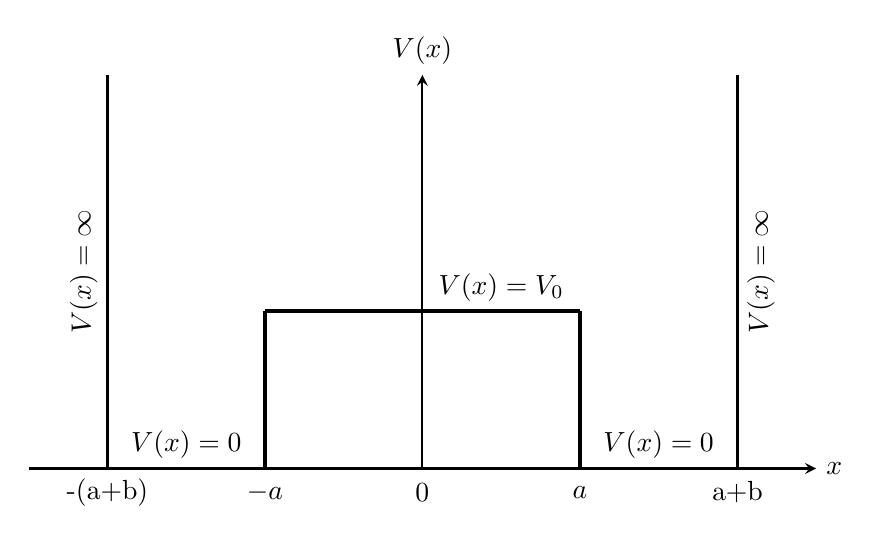
\begin{tikzpicture}[>=stealth, scale=1]
        \draw[->] (-5,0) -- (5,0) node[right] {$x$};
        \draw[->] (0,0) -- (0,5) node[above] {$V(x)$};
        \draw[very thick] (-2,2) -- (2,2);  
        \draw[very thick] (-2,0) -- (-2,2);      
        \draw[very thick] (2,0) -- (2,2);      
        \draw[very thick] (2,0) -- (4,0);
        \draw[very thick] (-4,0) -- (-2,0);
        \draw[very thick] (4,0) -- (4,5); 
        \draw[very thick] (-4,0) -- (-4,5);
        \node[rotate=90] at (-4.3,2.5) {$V(x)=\infty$};
        \node[rotate=90] at (4.3,2.5) {$V(x)=\infty$};
        \node at (0, -0.3) {0};
        \node at (2, -0.3) {$a$};
        \node at (-2, -0.3) {$-a$};
        \node at (3,0.3) {$V(x)=0$};
        \node at (-3,0.3) {$V(x)=0$};
        \node at (4,-0.3) {a+b};
        \node at (-4,-0.3) {-(a+b)};
        \node at (1,2.3) {$V(x)=V_0$};
    \end{tikzpicture}
\end{figure}

Since the potential is symmetric, the Hamiltonian $\oH$ commutes with the parity operator $\oPi$, i.e., $\comm{\oH}{\oPi} = 0$ \footnote{As we have disscussed in \cref{sec:parity_operator}}. Thus the energy eigenstates can be chosen to be simultaneous eigenstates of both $\oH$ and $\oPi$. The parity operator has eigenvalues $\pm 1$, corresponding to even and odd parity states, respectively. Therefore, the energy eigenstates can be classified into two categories: even parity states $\ket S$ (symmetric) and odd parity states $\ket A$ (antisymmetric).

By solving the time-independent Schrödinger equation for different regions, 
\begin{align}
    &- \frac{\hbar^2}{2m} \frac{\dd^2 \psi_1(x)}{\dd x^2}  = E_1 \psi_1(x) \quad a<\abs{x}<a+b\\
    &- \frac{\hbar^2}{2m} \frac{\dd^2 \psi_2(x)}{\dd x^2} + V_0 \psi_2(x) = E_2 \psi_2(x) \quad  \abs{x} < a 
\end{align}
here we can set $k = \sqrt{2mE}/\hbar$ and $\kappa = \sqrt{2m(E-V_0)}/\hbar $the area for $V(x) = \infty$ is infinite, thus the wave function must vanish in that region, i.e. at the coundary $\psi(a+b) = \psi(-(a+b)) = 0$. Actually we can just write one side since the wave function is either even or odd. The solutions are 
\begin{align}
    \psi_1(x) &= \begin{cases}
        A \cos(k x), & \text{even parity} \\
        C \sin(k x), & \text{odd parity} \\
\end{cases} \quad a< \abs{x} < a+b \\
    \psi_2(x) &= \begin{cases}
        B \cosh(\kappa x), & \text{even parity} \\
        D \sinh(\kappa x), & \text{odd parity} \\
    \end{cases} \quad \abs{x} < a
\end{align}
By the boundary condition mentioned above, we can obtain a general case for $\psi_1$
\begin{align}
    \psi_1(x) = \begin{cases}
        A \cos\left[k(x - a - b)\right], & \text{even parity} \\
        C \sin\left[k(x - a - b)\right], & \text{odd parity} \\
\end{cases} 
\end{align}
we disscuss the two cases separately.
\begin{itemize}
    \item \emph{Even parity}: The boundary condition of such case is $\psi_1(a)= \psi_2(a)$ and $\psi_1'(a) = \psi_2'(a)$. Applying these boundary conditions, we have
    \begin{align*}
        A \cos(kb) &= B \cosh(\kappa a) \\
        Ak \sin(kb) & = B \kappa \sinh(\kappa a)
    \end{align*}
    From these two, we can eliminate $A$ and $B$, obtaining the transcendental equation for even parity states:
    \begin{align}
        k \tan(kb) = \kappa \tanh(\kappa a) \label{eq:SDWP_quant1}
    \end{align}
    \item \emph{Odd parity}: The boundary condition of such case is $\psi_1(a)= \psi_2(a)$ and $\psi_1'(a) = \psi_2'(a)$. Applying these boundary conditions, we have
    \begin{align*}
        C \sin(kb) &= D \sinh(\kappa a) \\
        Ck \cos(kb) & = D \kappa \cosh(\kappa a)
    \end{align*}
    From these two, we can eliminate $C$ and $D$, obtaining the transcendental equation for odd parity states:
    \begin{align}
        k \cot(kb) = - \kappa \coth(\kappa a) \label{eq:SDWP_quant2}
    \end{align}
\end{itemize}
Such that we can find the symmetric and antisymmetric energy eigenvalues by solving \cref{eq:SDWP_quant1} and \cref{eq:SDWP_quant2} respectively. The corresponding wave functions are given by
\begin{align}
    \psi_S(x) &= \begin{cases}
        A \cos\left[k(x - a - b)\right], & a< \abs{x} < a+b \\
        B \cosh(\kappa x), & \abs{x} < a
    \end{cases} \\
    \psi_A(x) &= \begin{cases}
        C \sin\left[k(x - a - b)\right], & a< \abs{x} < a+b \\
        D \sinh(\kappa x), & \abs{x} < a
    \end{cases}
\end{align}
With the quantization condition \cref{eq:SDWP_quant1,eq:SDWP_quant2}, we can dissucss the energy eigenvalues. For a certain value of $V_0$, there is no way to express the ground state and the first excited state explicitly. However, if we set the barrier height $V_0 \to \infty$, the $\kappa$ goes to infinity, then the two equation reduce to 
\begin{align}
    &k \tan(kb) = \kappa \tanh(\kappa a) \to k \tan(kb) = \infty \quad \Longrightarrow \quad kb = \frac{\pi}{2}, \frac{3\pi}{2}, \frac{5\pi}{2}, \dots, \frac{(n+2)\pi}{2} \\
    &k \cot(kb) = - \kappa \coth(\kappa a) \to k \cot(kb) = -\infty \quad \Longrightarrow \quad kb = \pi, 2\pi, 3\pi, \dots , n\pi
\end{align}
But we need to relaize the fact that the wave functions are trapped in either well, thus the energy eigenvalues are doubly degenerate. The energy eigenvalues are given by
\begin{align}
    E_n = \frac{\hbar^2 k_n^2}{2m} = \frac{\hbar^2 \pi^2 n^2}{8 m b^2} \quad n = 1, 2, 3, \dots
\end{align}
with the corresponding wave functions
\begin{align}
    \psi_n(x) = \begin{cases}
        \sqrt{\frac{2}{b}} \cos\left(\frac{n \pi x}{2b}\right), & \text{for odd } n \\
        \sqrt{\frac{2}{b}} \sin\left(\frac{n \pi x}{2b}\right), & \text{for even } n \\
    \end{cases} \quad a < \abs{x} < a+b
\end{align}
\begin{figure}[h!]
    \centering
    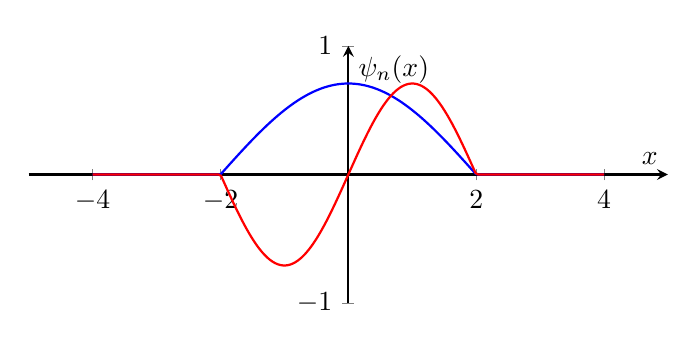
\begin{tikzpicture}
        \begin{axis}[
            axis lines = middle,
            xlabel = $x$,
            ylabel = {$\psi_n(x)$},
            ymin = -1,
            ymax = 1,
            xmin = -5,
            xmax = 5,
            xtick = {-4, -2, 0, 2, 4},
            ytick = {-1, 0, 1},
            domain = -4:4,
            samples = 200,
            width=0.8\textwidth,
            height=0.4\textwidth,
        ]
        \addplot[blue, thick] { (x < -2 || x > 2) * 0 + (x >= -2 && x <= 2) * (sqrt(2/4) * cos(deg(pi * 1 * x / (2 * 2)))) };
        \addplot[red, thick] { (x < -2 || x > 2) * 0 + (x >= -2 && x <= 2) * (sqrt(2/4) * sin(deg(pi * 2 * x / (2 * 2)))) };    
        \end{axis}
    \end{tikzpicture}
\end{figure}

It looks somehow weird that the energy eigenvalues are the same as a single infinite potential well of width $b$. This is because the two wells are completely isolated when $V_0 \to \infty$. In such case, there is no such even conditions anymore. So we juat take the single case solution here as the even one. When $V_0$ is finite, the wave functions in the two wells can overlap due to tunneling effect, leading to a splitting of the energy levels. The symmetric state $\ket S$ has a slightly lower energy than the antisymmetric state $\ket A$ due to constructive interference in the overlap region, while the antisymmetric state has a slightly higher energy due to destructive interference. This energy splitting is a hallmark of quantum tunneling in double well potentials.
We could disscuss the tunneling dynamics between the two wells as below.

Construct states $\ket R$ and $\ket L$ localized in the right and left wells respectively. 
\begin{align}
    \ket R &= \frac{1}{\sqrt 2} \left( \ket S + \ket A \right) \\
    \ket L &= \frac{1}{\sqrt 2} \left( \ket S - \ket A \right)
\end{align}
S,A denoting the symmetric and antisymmetric states. The tunneling between the two wells can be described by time evolution of the states:
\begin{align}
    \ket R(t) &= \frac{1}{\sqrt 2} \left( \ee^{- \ii E_S t / \hbar} \ket S + \ee^{- \ii E_A t / \hbar} \ket A \right) \\
    &= \frac{1}{\sqrt 2} \ee^{- \ii (E_S + E_A) t / 2 \hbar} \left( \ee^{- \ii (E_S - E_A) t / 2 \hbar} \ket S + \ee^{\ii (E_S - E_A) t / 2 \hbar} \ket A \right) \\
    &= \ee^{- \ii (E_S + E_A) t / 2 \hbar} \left[ \cos \left( \frac{E_A - E_S}{2 \hbar} t \right) \ket R - \ii \sin \left( \frac{E_A - E_S}{2 \hbar} t \right) \ket L \right]
\end{align}
At time $t = T/2$ determined by from above equation, we have
\begin{align}
    \ket R(T/2) = - \ii \ee^{- \ii (E_S + E_A) T / 4 \hbar} \ket L
\end{align}
indicating that the particle initially localized in the right well has tunneled to the left well 
\begin{align}
    T = \frac{2 \pi \hbar}{E_A - E_S}
\end{align}
\begin{ex}
    ammonia molecule NH$_3$ has a pyramidal structure with the nitrogen atom able to tunnel through the plane formed by the three hydrogen atoms. This tunneling leads to an inversion of the molecule, which can be modeled as a particle in a double well potential. The two wells correspond to the nitrogen atom being above or below the plane of hydrogen atoms. The energy splitting between the symmetric and antisymmetric states due to tunneling results in a characteristic frequency of inversion, which can be observed spectroscopically. This phenomenon is a classic example of quantum tunneling in molecular systems.
\end{ex}
\begin{figure}[h!]
    \centering
    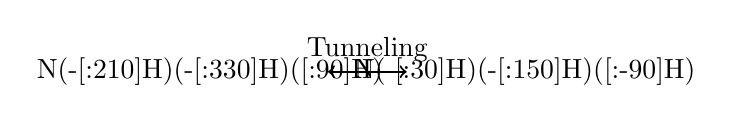
\begin{tikzpicture}
        % 左：N 在下方（H3 朝上）
        \node at (0,0)
            {\chemfig{N(-[:210]H)(-[:330]H)([:90]H)}};
        % 右：N 在上方（H3 朝下）
        \node at (4,0)
            {\chemfig{N(-[:30]H)(-[:150]H)([:-90]H)}};
        % 双箭头
        \draw[<->] (1.5,0) -- (2.5,0)
            node[midway,above]{Tunneling};
    \end{tikzpicture}
    \caption{Inversion of ammonia NH$_3$ due to tunneling of the N atom through the plane of H atoms.}
\end{figure}

The energy and parity eigenstates are superpositions of the localized states: 
\begin{align}
    \ket S &= \frac{1}{\sqrt 2} \left( \upket + \downket \right) \\
    \ket A &= \frac{1}{\sqrt 2} \left( \upket - \downket \right)
\end{align}

Naturally occuring organic molecules, such as amino acids, which are of R-type or L-type only. Such molecules with a definite handedness are called optical isomers. The oscillation time $(10^4 \text{ to } 10^6)$ is infinite for practical. Chiral can be determined by the polarized light rotation experiment. A synthesis in the labotatory yields equal amonut of $R-$ and $L-$ type

\emph{This is also Strum-Liouville theory}

\subsection{Parity Selection Rule}

Consider parity eigenstates $\ket \alpha$ and $\ket \alpha$ with eigenvalues $\lambda_{\alpha}, \lambda_{\beta} = \pm 1$. 
\begin{align}
    \oPi \ket \alpha = \lambda_{\alpha} \ket \alpha, \quad \oPi \ket \beta = \lambda_{\beta} \ket \beta
\end{align}
Consider the matrix element of potition operator $\ox$ between these two states:
\begin{align}
    \bra \alpha \ox \ket \beta &= \bra \alpha \oPi^ \dag \ox \oPi \ket \beta \notag \\
    &= - \bra \alpha \ox \ket \beta \notag \\
    & = 0 \quad \text{if } \lambda_{\alpha} \lambda_{\beta} = 1
\end{align}
But the reality is that $\ox$ is an odd operator under parity transformation, i.e., $\oPi^ \dag \ox \oPi = - \ox$. Thus the matrix element $\bra \alpha \ox \ket \beta$ vanishes unless the two states have opposite parity, i.e., $\lambda_{\alpha} \lambda_{\beta} = -1$. This result is known as the parity selection rule, which states that transitions between states of the same parity are forbidden for operators that are odd under parity transformation.

\subsection{Parity nonconservation}

$\beta$-decay: neutron decays into a proton, an electron and an anti-neutrino. The proton and neutron form an isospin doublet, and the weak interaction responsible for $\beta$-decay violates parity symmetry. This was first experimentally confirmed in the Wu experiment in 1957, which demonstrated that the distribution of emitted electrons in the decay of polarized cobalt-60 nuclei was not symmetric with respect to spatial inversion. This discovery had profound implications for our understanding of fundamental symmetries in physics and led to the realization that the weak interaction is not invariant under parity transformation. 

\newpage
\subsection{Lattice Translation}

Consider a periodic potential in 1d, with $V(x) = V(x+a)$, as shown in \cref{fig:periodic_lattics}.

\begin{figure}[h!]
    \centering
    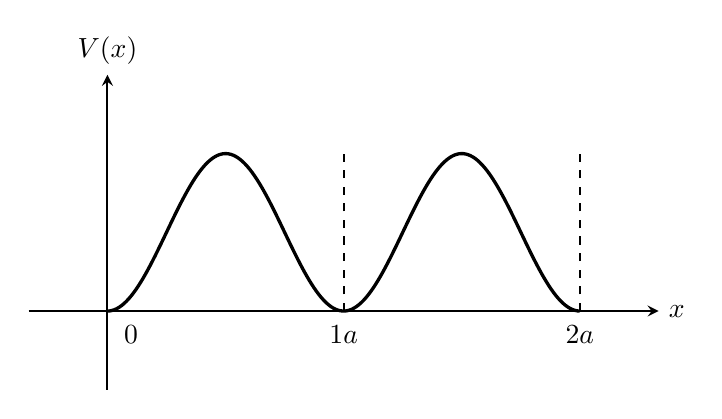
\begin{tikzpicture}[>=stealth, scale=1]
        \draw[->] (-1,0) -- (7,0) node[right] {$x$};
        \draw[->] (0,-1) -- (0,3) node[above] {$V(x)$};
        \node at (0.3,-0.3) {0};
        \draw[very thick, domain=0:6, samples=200] plot (\x, {2*sin(deg(pi*\x/3))^2});
        \foreach \i in {1,2} {
            \draw[dashed] (3*\i,0) -- (3*\i,2);
            \node at (3*\i, -0.3) {\( \i a \)};
        }
    \end{tikzpicture}
    \caption{Periodic potential with period $a$.}
    \label{fig:periodic_lattics}
\end{figure}

Such a potential may describe the motion of an electron in a chain of regularly spcaed ions. In general the Hamiltonian is not invariant under a translation by an arbitrary length $l$ as the definition of a translation operaotr in \cref{sec:translation_symmetry}. However, the Hamiltonian is invariant under a translation by an integer multiple of the lattice constant $a$.
This is because the potential satisfies $V(x+na) = V(x)$ for any integer $n$. As a result, the energy eigenstates of the Hamiltonian can be chosen to be simultaneous eigenstates of the lattice translation operator $\oT(na)$. 
\begin{align}
    &\oT_a^ \dag V(\ox) \oT_a = V (\ox+a) = V(\ox)  \\
    \implies & {\oT_a^ {\dag n}} V(\ox) {\oT_a}^n = V(\ox +na) = V(\ox)
\end{align}
The kinetic energy in Hamiltonian is invariant under arbitrary displacement, the entire Hamiltonian satisfies
\begin{align}
    \oT_a^ \dag \oH \oT_a = \oH 
\end{align}
And we know that the translation operator is an unitary operator 
\begin{align}
    \oH \oT_a - \oT_a \oH = 0 \implies \comm{\oH}{\oT_a} = 0
\end{align}
Such that the Hamiltonian and Lattice Translation Operators can be simultaneously diagonalized for this reason. 

Now consider a periodic potential with infinitely high boundaries. 
\begin{figure}[h!]
    \centering
    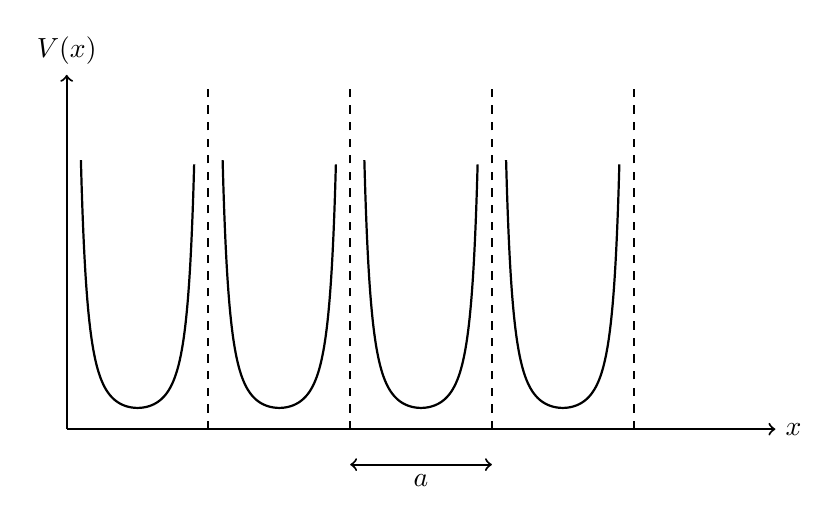
\begin{tikzpicture}[scale=0.9]

  % 坐标轴
  \draw[->] (0,0) -- (10,0) node[right] {$x$};
  \draw[->] (0,0) -- (0,5) node[above] {$V(x)$};

  % 晶格周期边界（虚线）
  \foreach \x in {2,4,6,8}{
    \draw[dashed] (\x,0) -- (\x,4.8);
  }

  % 每个势阱：在边界处势能发散（用 1/(x-x_0)^2 型函数表示）
    \draw[thick,smooth,domain=2.2:3.8,samples=150]
    plot (\x,{0.15*(1/((\x-2)^2)+1/((4-\x)^2))});
    \draw[thick,smooth,domain=4.2:5.8,samples=150]
    plot (\x,{0.15*(1/((\x-4)^2)+1/((6-\x)^2))});
    \draw[thick,smooth,domain=6.2:7.8,samples=150]
    plot (\x,{0.15*(1/((\x-6)^2)+1/((8-\x)^2))});
    \draw[thick,smooth,domain=0.2:1.8,samples=150]
    plot (\x,{0.15*(1/((\x-0)^2)+1/((2-\x)^2))});
  % 周期 a 标注
  \draw[<->] (4,-0.5) -- (6,-0.5)
    node[midway,below] {$a$};

    \end{tikzpicture}
    \caption{Periodic potential with infinitely high boundaries.}
    \label{fig:periodic_lattics_infinite}
\end{figure}

A particle located at the lattice site $n$ is a ground state of the Hamiltonian. We denote this state by $\ket{n}$, $\oH \ket{n} = E_0 \ket{n}$. The wave function $\braket{x'|n}$ is finite only on the n-th lattice site\footnote{We can see that the potential will go to infinite at each edge of the lattice}. $\ket{n}$ is not an eigenstate of $\oT_a$: 
\begin{align}
    \oT_a \ket{n} = \ket{n+1}
\end{align}
This is possible as the energy eigenstates of the Hamiltonian can be degenerate. And because of the potential well is infinitely high at the boundaries, so each lattice site is isolated. Consider a new state defined as 
\begin{align}
    \ket{\theta} \equiv \sum_{n=-\infty}^{\infty} \ee^{\ii n \theta} \ket{n} \quad \theta \in [-\pi, \pi]
\end{align}
The choice of the phase factor $\ee^{\ii n \theta}$ is to ensure that $\ket{\theta}$ is an eigenstate of the lattice translation operator $\oT_a$:
\begin{align}
    \oT_a \ket{\theta} &= \sum_{n=-\infty}^{\infty} \ee^{\ii n \theta} \oT_a \ket{n} = \sum_{n=-\infty}^{\infty} \ee^{\ii n \theta} \ket{n+1} \notag \\
    &= \ee^{- \ii \theta} \sum_{m=-\infty}^{\infty} \ee^{\ii m \theta} \ket{m} = \ee^{- \ii \theta} \ket{\theta}
\end{align}
For last line we have made a change of variable $m = n+1$. Thus $\ket{\theta}$ is an eigenstate of $\oT_a$ with eigenvalue $\ee^{- \ii \theta}$. Since $\oH \ket{n} = E_0 \ket{n}$ for all $n$, we have 
\begin{align}
    \oH \ket{\theta} &= \sum_{n=-\infty}^{\infty} \ee^{\ii n \theta} \oH \ket{n} = E_0 \sum_{n=-\infty}^{\infty} \ee^{\ii n \theta} \ket{n} = E_0 \ket{\theta}
\end{align}
Thus $\ket{\theta}$ is also an eigenstate of the Hamiltonian with eigenvalue $E_0$. Therefore, we have constructed a set of simultaneous eigenstates of both the Hamiltonian and the lattice translation operator, labeled by the continuous parameter $\theta$. The eigenvalue of the lattice translation operator is $\ee^{- \ii \theta}$, which lies on the unit circle in the complex plane.
\begin{figure}[h!]
    \centering
    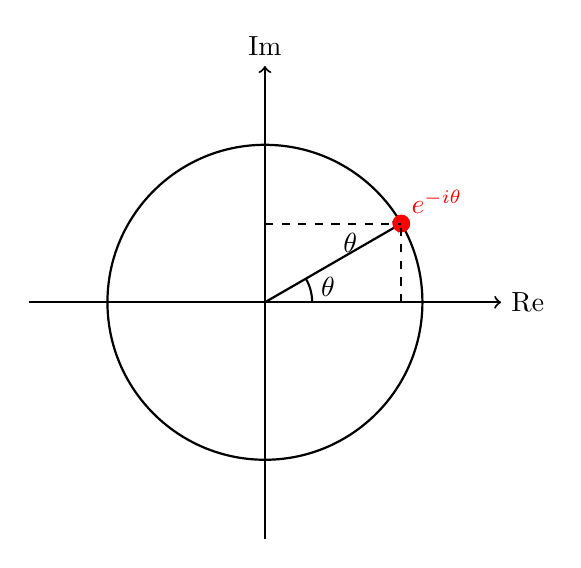
\begin{tikzpicture}[scale=2]
        % Draw the unit circle
        \draw[thick] (0,0) circle(1);
        
        % Draw the axes
        \draw[->] (-1.5,0) -- (1.5,0) node[right] {Re};
        \draw[->] (0,-1.5) -- (0,1.5) node[above] {Im};
        
        % Draw the angle theta
        \draw[thick,->] (0,0) -- (0.866,0.5) node[midway, above right] {$\theta$};
        
        % Mark the point on the unit circle
        \filldraw[red] (0.866,0.5) circle(0.05) node[above right] {$e^{-i\theta}$};
        
        % Draw dashed lines to axes
        \draw[dashed] (0.866,0) -- (0.866,0.5);
        \draw[dashed] (0,0.5) -- (0.866,0.5);
        
        % Label the angle
        \draw (0.3,0) arc(0:30:0.3);
        \node at (0.4,0.1) {$\theta$};
    \end{tikzpicture}
    \caption{Eigenvalue $e^{-i\theta}$ of the lattice translation operator $\oT_a$ on the complex unit circle.}
\end{figure}

But for this case, the wave fucntions are only localized at each lattice site, there is no overlap between different sites, thus the energy eigenvalue is degenerate and independent of $\theta$. In a more realistic scenario where the potential wells have finite depth, as shown in \cref{fig:Lattice_finite_wavefunction} , the wave functions can overlap between neighboring lattice sites due to quantum tunneling(or to say the wavefunction have tails extending to neighboring sites). This overlap leads to a dependence of the energy eigenvalues on the parameter $\theta$, resulting in the formation of energy bands characteristic of electrons in crystalline solids.

\begin{figure}[h!]
    \centering
    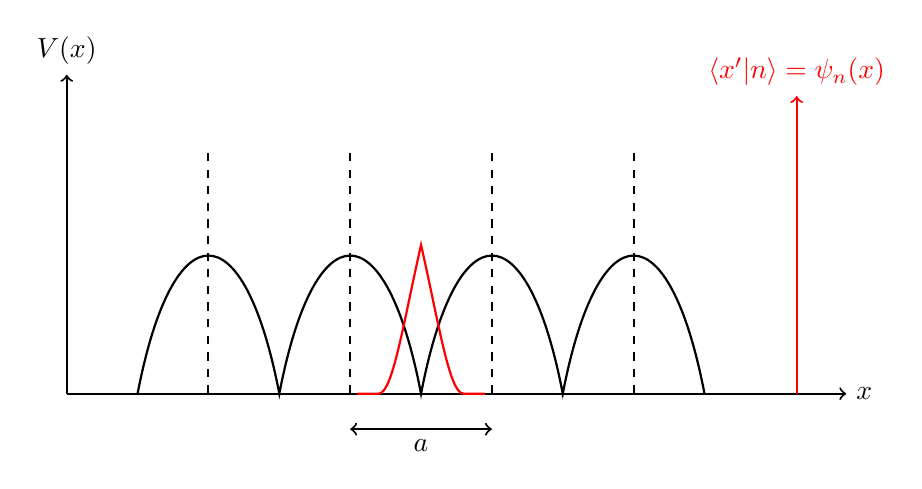
\begin{tikzpicture}[scale=0.9]

  % axes
  \draw[->] (0,0) -- (11,0) node[right] {$x$};
  \draw[->] (0,0) -- (0,4.5) node[above] {$V(x)$};

  % periodic potential (schematic bumps)
  \draw[thick]
    (1,0) .. controls (1.5,2.6) and (2.5,2.6) .. (3,0)
          .. controls (3.5,2.6) and (4.5,2.6) .. (5,0)
          .. controls (5.5,2.6) and (6.5,2.6) .. (7,0)
          .. controls (7.5,2.6) and (8.5,2.6) .. (9,0);

  % cell boundaries (dashed)
  \foreach \x in {2,4,6,8}{
    \draw[dashed] (\x,0) -- (\x,3.4);
  }

  % localized wave function in one well
  \draw[red,thick]
    (4.1,0) -- (4.4,0)
      .. controls (4.6,0)   and (4.75,1.0) .. (5,2.1)
      .. controls (5.25,1.0) and (5.4,0)   .. (5.6,0)
    -- (5.9,0);

  % lattice spacing a
  \draw[<->] (4,-0.5) -- (6,-0.5)
    node[midway,below] {$a$};

  % vertical axis for wave function
  \draw[->,red] (10.3,0) -- (10.3,4.2)
    node[above] {$\langle x'|n\rangle = \psi_n(x)$};

\end{tikzpicture}
\caption{Periodic finite lattice potential and wave function on lattice n}
\label{fig:Lattice_finite_wavefunction}
\end{figure}

The diagonal matrix elements of the Hamiltonian $\bra{n} \oH \ket{n} = E_0$ must be all equal as the translation invariance. 
We suppose that the only non-diagnoal elements of importance are the one connecting immediate neighbors.
\begin{align}
    \bra{n'} \oH \ket{n} \geq 0 \text{ iff } n'=n, n \pm 1
\end{align}
Such assumption is called the \emph{tight-binding approximation}, which is valid when the overlap between wave functions on non-neighboring sites is negligible, also could be written as 
\begin{align}
    \bra{n+1} \oH \ket{n} = - \Delta
\end{align}
which is independent of $n$ due to translation invariance. Under this approximation, we can write the action of the Hamiltonian on the state $\ket{n}$ as
\begin{align}
    \oH \ket n = E_0 \ket n - \Delta \ket {n+1} - \Delta \ket {n-1}
\end{align}
We can now again form the linear combination state $\ket \theta$ as before, 
\begin{align}
    \ket{\theta} = \sum_n \ee^{\ii n \theta} \ket n \quad \& \quad \oT_a \ket{\theta} = \ee^{- \ii \theta} \ket{\theta}
\end{align}
Applying the Hamiltonian to $\ket \theta$, we have
\begin{align}
    \oH \ket \theta &= \sum_n \ee^{\ii n \theta} \oH \ket n \notag \\
    &= \sum_n \ee^{\ii n \theta} \left( E_0 \ket n - \Delta \ket {n+1} - \Delta \ket {n-1} \right) \notag \\
    &= E_0 \sum_n \ee^{\ii n \theta} \ket n - \Delta \sum_n \ee^{\ii n \theta} \ket {n+1} - \Delta \sum_n \ee^{\ii n \theta} \ket {n-1} \notag \\
    &= E_0 \ket{\theta} - \Delta \ee^{- \ii \theta} \sum_m \ee^{\ii m \theta} \ket m - \Delta \ee^{\ii \theta} \sum_l \ee^{\ii p \theta} \ket l \notag \\
    &= E_0 \ket{\theta} - \Delta (\ee^{- \ii \theta} + \ee^{\ii \theta}) \ket{\theta} \\ 
    &= \left[ E_0 - 2 \Delta \cos(\theta) \right] \ket{\theta}
\end{align}
The eigenstate depend on the parameter $\theta$. The degeneracy is lifted, and we have a contineous spectrum of eigenvalues between $E_0 - 2 \Delta$ and $E_0 + 2 \Delta$. 

Consider the wavefunction $\braket{x'|\theta}$. For the translated state $\oT_a \theta$, we have 
\begin{align}
    \bra{x'} \oT_a \ket{\theta} & = \left( \bra{x'} \oT_{-a}^ \dag \right)\ket{\theta} \notag \\
    &= \braket{x'-a|\theta} 
\end{align}
Together with the eigenvalue equation of $\oT_a$, we have
\begin{align}
    \braket{x'-a|\theta} = \ee^{- \ii \theta} \braket{x'|\theta}
\end{align}
We find a solution by making the ansatz
\begin{align}
    \braket{x'|\theta} = \ee^{\ii k x'} u_k(x') \text{ with } \theta = k a \text{ and } u_k(x'\pm a) = u_k(x')
\end{align}
We can verify that this ansatz satisfies the above equation: 
\begin{align}
    \braket{x'-a|\theta} &= \ee^{\ii k (x'-a)} u_k(x'-a) \notag \\
    &= \ee^{\ii k (x'-a)} u_k(x') \notag \\
    &= \ee^{- \ii k a} \ee^{\ii k x'} u_k(x') \notag \\
    &= \ee^{- \ii k a} \braket{x'|\theta}
\end{align}
For wave functions in a periodic potential, we therefore find the condition known as \emph{Bloch Theorem}: 
\begin{theorem}[Bloch Theorem]
    The energy eigenstates of a particle in a periodic potential can be expressed in the form
    \begin{align}
        \psi_k(x) = \braket{x|k} = \ee^{\ii k x} u_k(x)
    \end{align}
    where $u_k(x)$ is a function with the same periodicity as the potential, i.e., $u_k(x+a) = u_k(x)$ for all $x$. Here, $k$ is the crystal momentum, which lies within the first Brillouin zone, typically defined as $-\pi/a \leq k < \pi/a$.
\end{theorem}




\newpage






\subsection{Time-Reversal Discrete Symmetry}

The conception of time-reversal is sound somehow scientific puuzle. What dose it exactly mean? Let us consider a different example: position-reversal. Consider a particle move a along a curve(also its trajectory) which is parameterized by time $t$. At time $t=0$, we let the  paricle stop and reverse its motion, the position and momentum is then be $x|_{t=0_-} = -x|_{t=0_+} $
, $p|_{t=0_+} = p|_{t=0_-}$. The particle then move back along the same curve but in the opposite direction. 
\begin{figure}[h!]
    \centering
    \tikzset{every picture/.style={line width=0.75pt}} %set default line width to 0.75pt        

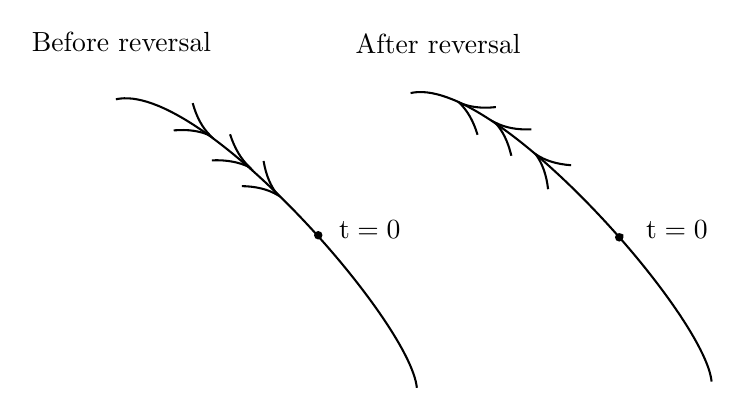
\begin{tikzpicture}[x=0.75pt,y=0.75pt,yscale=-1,xscale=1]
%uncomment if require: \path (0,300); %set diagram left start at 0, and has height of 300

%Curve Lines [id:da5488504090671414] 
\draw    (163,113) .. controls (203,104) and (305,220) .. (308,252) ;
%Curve Lines [id:da023649926549646594] 
\draw    (305,110) .. controls (345,101) and (447,217) .. (450,249) ;
\draw   (190.86,127.99) .. controls (197.77,127.39) and (203.68,128.26) .. (208.56,130.57) .. controls (204.7,126.8) and (201.85,121.55) .. (200.01,114.86) ;
\draw   (363.21,127.48) .. controls (356.28,127.79) and (350.42,126.67) .. (345.64,124.15) .. controls (349.34,128.09) and (351.97,133.45) .. (353.52,140.21) ;
\draw   (209.26,142.42) .. controls (216.27,142.12) and (222.31,143.23) .. (227.38,145.72) .. controls (223.28,141.83) and (220.16,136.54) .. (218.01,129.86) ;
\draw   (223.72,154.84) .. controls (230.65,154.95) and (236.44,156.42) .. (241.06,159.22) .. controls (237.6,155.07) and (235.3,149.56) .. (234.16,142.72) ;
\draw   (346.09,116.76) .. controls (339.19,117.51) and (333.27,116.78) .. (328.34,114.57) .. controls (332.28,118.26) and (335.25,123.44) .. (337.24,130.09) ;
\draw   (382.31,144.77) .. controls (375.39,144.28) and (369.69,142.51) .. (365.23,139.46) .. controls (368.46,143.79) and (370.46,149.42) .. (371.23,156.31) ;
%Shape: Circle [id:dp870416844684753] 
\draw  [fill={rgb, 255:red, 0; green, 0; blue, 0 }  ,fill opacity=1 ] (259,178.5) .. controls (259,177.67) and (259.67,177) .. (260.5,177) .. controls (261.33,177) and (262,177.67) .. (262,178.5) .. controls (262,179.33) and (261.33,180) .. (260.5,180) .. controls (259.67,180) and (259,179.33) .. (259,178.5) -- cycle ;
%Shape: Circle [id:dp9542782425706763] 
\draw  [fill={rgb, 255:red, 0; green, 0; blue, 0 }  ,fill opacity=1 ] (407,178.5) .. controls (407,178.67) and (406.33,178) .. (405.5,178) .. controls (404.67,178) and (404,178.67) .. (404,179.5) .. controls (404,180.33) and (404.67,181) .. (405.5,181) .. controls (406.33,181) and (407,180.33) .. (407,179.5) -- cycle ;

% Text Node
\draw (269,170) node [anchor=north west][inner sep=0.75pt]    {$\mathrm{t} =0$};
% Text Node
\draw (417,170) node [anchor=north west][inner sep=0.75pt]    {$\mathrm{t} =0$};
% Text Node
\draw (121,79) node [anchor=north west][inner sep=0.75pt]   [align=left] {Before reversal};
% Text Node
\draw (277,80) node [anchor=north west][inner sep=0.75pt]   [align=left] {After reversal};


\end{tikzpicture}
\caption{Position-reversal of a particle along its trajectory.}
\end{figure}

Generally speaking, if $x(t)$ is a solution of Newton's equation of motion, then so is $-x(-t)$.
\begin{align}
    t'=t \implies \ddx{t'} = - \ddx{t} \implies \ddxx{}{{t'}} = \ddxx{}{t}
\end{align}

We now consider time-reversal, with a similar consideration by Schrödinger equation \cref{eq:time_dependent_schrodinger_equation}. When we have a solution $\psi(x,t)$, the time-reversed solution is given by $\psi^*(x,-t)$. There is a bit difference here compared to Newton's equation of motion, now let's see why we need to take the complex conjugate. Take the so called pre-time-reversal operator $\oT_p$ which just simply reverse the time $t \to -t$, we have the time-dependent Schrödinger equation as
\begin{align*}
    \ii \hbar \pdv{\psi(x,-t)}{(-t)} = \oH \psi(x,-t) \\
    - \ii \hbar \pdv{\psi(x,-t)}{t} = \oH \psi(x,-t)
\end{align*}
This is not the concrete time-reversed Schrödinger equation, as the sign in front of the imaginary unit is different. To fix this, we need to take the complex conjugate of the wave function, leading to the true time-reversed wave function $\psi^*(x,-t)$. Taking the complex conjugate of the above equation, we have
\begin{align*}
    \ii \hbar \pdv{\psi^*(x,-t)}{t} = \oH \psi^*(x,-t)
\end{align*}

Now we have the correct time-reversed Schrödinger equation. Thus the time-reversal operator $\oThe$ can cause a transformation on the wave function not just by reversing the time, but also taking the complex conjugate:
\begin{align*}
    \oThe \psi(x,t) = \psi^*(x,-t)
\end{align*}

Before we proceed to find the eigenvalue and eigenstate of the time-reversal operator, we first check whether the time-reversal operator is a linear operator. Consider a linear combination of two wave functions $\psi_1(x,t)$ and $\psi_2(x,t)$, we have
\begin{align*}
    \oThe \left( a \psi_1(x,t) + b \psi_2(x,t) \right) &= a \psi_1^*(x,-t) + b \psi_2^*(x,-t) \\
    &\neq a \oThe \psi_1(x,t) + b \oThe \psi_2(x,t)
\end{align*}
Thus the time-reversal operator is not a linear operator, but an anti-linear operator due to the complex conjugation.

As we are actually talking about the symmetry. So let us introduce a important theorem here.
\begin{theorem}[Wigner's Theorem]
    Any symmetry transformation in quantum mechanics can be represented by either a unitary operator or an anti-unitary operator acting on the Hilbert space of states.
\end{theorem}
\begin{proof}
    Consider a symmetry transformation $\oS$ that maps state vectors in the Hilbert space to other state vectors. 
    By definition of a symmetry in quantum mechanics it must preserve all transition probabilities, i.e.\ for any two state vectors $\ket{\psi}$ and $\ket{\phi}$ we require
    \begin{align*}
        \abs{\braket{\psi|\phi}}^2 = \abs{\braket{\oS\psi|\oS\phi}}^2 .
    \end{align*}
    In particular, this implies that norms are preserved,
    \begin{align*}
        \braket{\psi|\psi} = \braket{\oS\psi|\oS\psi},
    \end{align*}
    and that the absolute value of every inner product is unchanged. 
    Physically, the operation $\oS$ may change phases, but it cannot change any probability.

    From this preservation of the inner product structure one can show that there are only two possibilities for how $\oS$ acts on superpositions of states: for any complex numbers $a,b$ and any states $\ket{\psi},\ket{\phi}$,
    \begin{align}
        \oS \bigl(a \ket{\psi} + b \ket{\phi}\bigr)
        = a\, \oS \ket{\psi} + b\, \oS \ket{\phi}
        \label{eq:wigner-linear}
    \end{align}
    (the \emph{linear} case), or
    \begin{align}
        \oS \bigl(a \ket{\psi} + b \ket{\phi}\bigr)
        = a^* \oS \ket{\psi} + b^* \oS \ket{\phi}
        \label{eq:wigner-antilinear}
    \end{align}
    (the \emph{anti-linear} case).  
    The idea of the proof is that, since probabilities for all superpositions must be preserved, the relative phases in a superposition can only be kept as they are [case \eqref{eq:wigner-linear}] or be complex–conjugated [case \eqref{eq:wigner-antilinear}]. 
    No other dependence on $a$ and $b$ is compatible with the requirement that all transition probabilities remain the same.

    Next we choose an orthonormal basis $\{\ket{e_i}\}$ of the Hilbert space.  
    Because $\oS$ preserves norms and the absolute values of inner products, the transformed vectors $\{\oS\ket{e_i}\}$ also form an orthonormal set. 
    We now define an operator by its action on this basis.

    If $\oS$ is linear as in \eqref{eq:wigner-linear}, we define a linear operator $\oU$ by
    \begin{align*}
        \oU \ket{e_i} = \oS \ket{e_i} .
    \end{align*}
    Extending $\oU$ linearly to the whole space, we have for arbitrary states
    \begin{align*}
        \braket{\oU\psi|\oU\phi} = \braket{\psi|\phi},
    \end{align*}
    since the matrix elements in the basis $\{\ket{e_i}\}$ are unchanged. 
    Thus $\oU$ is a norm– and inner–product–preserving linear map, i.e.\ a unitary operator.

    If instead $\oS$ is anti-linear as in \eqref{eq:wigner-antilinear}, we define an anti-linear operator $\oA$ by
    \begin{align*}
        \oA \ket{e_i} = \oS \ket{e_i} ,
    \end{align*}
    and extend it anti-linearly. 
    One then finds
    \begin{align*}
        \braket{\oA\psi|\oA\phi} = \braket{\psi|\phi}^* ,
    \end{align*}
    so $\oA$ preserves norms and complex–conjugates inner products. 
    Such an operator is called \emph{anti-unitary}.

    In summary, any symmetry transformation $\oS$ that preserves transition probabilities can be represented on the Hilbert space either by a unitary operator $\oU$ or by an anti-unitary operator $\oA$. 
    This is Wigner's theorem.
\end{proof}
Wigner's theorem tells us that symmetries in quantum mechanics can be represented by operators that preserve the inner product structure of the Hilbert space, either through linear (unitary) or anti-linear (anti-unitary) transformations. Since the time-reversal operator is anti-linear, it must be represented by an anti-unitary operator according to Wigner's theorem.

For this reason, the time-reversal operator $\oThe$ is an anti-unitary operator can be expressed as the product of a unitary operator $\oU$ and the complex conjugation operator $\oK$, i.e.,
\begin{align}
    \oThe = \oU \oK
\end{align}

where $\oK$ acts on a vector $c\ket{\psi}$ with $c \in \C$ by taking its complex conjugate:
\begin{align}
    \oK \left( c \ket{\psi} \right) = c^* \ket{\psi}
\end{align}
If $\ket{\psi}$ could be expanded in a basis $\{ \ket{n} \}$ as $\ket{\psi} = \sum_n \ket{n} \braket{n|\psi}$, then the action of $\oK$ on $\ket{\psi}$ is given by
\begin{align}
    \oK \ket{\psi} = \sum_n \braket{n|\psi}^* \ket{n} \label{eq:complex_conjugation_operator}
\end{align}

Let us check the anti-linearity of $\oThe$
\begin{align*}
    \oThe \left(c_1 \kps + c_2 \kph\right) &= \oU \oK \left(c_1 \kps + c_2 \kph\right) \\
    &= \oU \left(c_1^* \oK \kps + c_2^* \oK \kph\right) \\
    &= c_1^* \oU \oK \kps + c_2^* \oU \oK \kph \\
    &= c_1^* \oThe \kps + c_2^* \oThe \kph
\end{align*}

As the form \cref{eq:complex_conjugation_operator}, we can see that it is safer to not consider the action of $\oThe$ on bras of the Hermitian adjoint $\oThe^ \dag$. Consider the transformed vector 
\begin{align*}
    &\oThe \kps = \sum_n \braket{n|\psi}^* \oU \ket{n} = \sum_n \braket{\psi|n} \oU \ket{n} \\
    &\oThe \kph = \sum_n \braket{n|\phi}^* \oU \ket{n} = \sum_n \braket{\phi|n} \oU \ket{n} \\
    \implies & \braket{\oThe \psi|\oThe \phi} = \sum_{m,n} \braket{\psi|m}^* \braket{n|\phi} \bra{m} \oU^ \dag \oU \ket{n} \\
    &= \sum_{m,n} \braket{\psi|m}^* \braket{n|\phi} \delta_{mn} = \sum_n \braket{\psi|n}^* \braket{n|\phi} \\
    &= \left( \sum_n \braket{n|\psi} \braket{\phi|n} \right)^* = \braket{\phi|\psi}^*
\end{align*}
Now we could say, an anti-unitary operator $\oThe$ satisfies such kind of decomposition of inner product.
\subsection{Time-Reversal Operator}

We now consider the time-reversal operator $\oThe$ in more detail. The time-reversal operator could be considered by time evolution operator. Consider a infinitesimal $\delta t$ we have
\begin{align*}
    \ket{\psi;t_0=0,t= \delta t} = \left(1 - \frac{\ii \oH}{\hbar} \delta t\right)
\end{align*}
with an initial state $\ket{\psi;0,0} = \ket{\psi}$. The time evolution of the time-reversed state is given by
\begin{align*}
    \left(1 - \frac{\ii \oH}{\hbar} \delta\right) \oThe \kps
\end{align*}
If the motion is symmetry under time-reversal, then the state $\oThe \ket{\psi; t_0 =0, t= \delta t}$ is the same state as $\ket{\psi; t_0 =0, t= - \delta t}$, we have
\begin{align*}
    \oThe \left(1 - \frac{\ii \oH}{\hbar} \delta t\right) \kps = \left(1 - \frac{\ii \oH}{\hbar} \delta t\right) \oThe \kps
\end{align*}
If the relation is true for arbitrary $\ket{\psi}$, if $\oThe$ is unitary we have
\begin{align*}
    - \ii \oH \oThe = \ii \oThe \oH \implies \anticomm{\oH}{\oThe} = 0
\end{align*}

Consider now an energy eigenstate $\ket n$ with eigenvalue $E_n$. Then, the time reversed state $\oThe \ket{n}$ satisfies 
\begin{align*}
    \oH \oThe \ket{n} &= - \oThe \oH \ket{n} \notag \\
    &= - E_n \oThe \ket{n}
\end{align*}

Thus $\oThe \ket{n}$ is also an energy eigenstate with the same eigenvalue $-E_n$. This is not possible even in the elementary case of a free particle: the spectrum $\frac{\hbar^2 k^2 }{2m}$ is positive semidefinite and thus not contain negative eigenvalues.
Such that the time-reversal operator $\oThe$ must be anti-unitary. Then 
\begin{align*}
    - \ii \oH \oThe = \oThe \ii \oH = - \ii \oThe \oH \implies \comm{\oH}{\oThe} = 0
\end{align*}
The Hamiltonian is commutative with the time-reversal operator. Also called time-reversal symmetry of Hamiltonian.

Now consider a general operator $\oO$, and want to find how it transforms under time-reversal. Firstly give the expression and then proof it. 
\begin{align}
    \bra{\phi} \oO \kps = \bra{\oThe \psi} \oThe \oO \oThe^{-1} \ket{\oThe \phi} \label{eq:time_reversal_operator_transformation} 
\end{align}
\begin{proof}
    Define $\ket{\phi'} \equiv \oO^ \dag \ket{\phi}$, the corresponding bra is $\bra{\phi'} = \bra{\phi} \oO$. Then using $\ket{ \oThe\phi'} = \oThe \ket{\phi'}$, we have
    \begin{align*}
        \bra{\phi} \oO \kps & = \braket{\phi'|\psi} = \braket{\oThe \psi| \oThe \phi'} \\
        &= \bra{\oThe \psi} \oThe \oO^ \dag \ket{\phi} = \bra{\oThe \psi} \oThe \oO^ \dag \oThe^{-1} \ket{\oThe \phi} 
    \end{align*}
    For the first line we have used the anti-unitary property of $\oThe$.
\end{proof}

Such that, given a Hermitian operator $\oA$, we find 
\begin{align}
    \bra{\phi} \oA \kps = \bra{\oThe \psi} \oThe \oA \oThe^{-1} \ket{\oThe \phi} \label{eq:trs_hermitian}
\end{align}
We define an oberservable $\oA$ to be even or odd under time-reversal according to whether the upper or lower sign in the following relation holds:
\begin{align*}
    \oThe \oA \oThe^{-1} = \pm \oA
\end{align*}
Plug in this realtion to \cref{eq:trs_hermitian}, we have
\begin{align*}
    \bra{\phi} \oA \kps = \pm \bra{\oThe \psi} \oA \ket{\oThe \phi}
\end{align*}

For example, the position operator $\ox$ is even under time-reversal:
\begin{align}
    \oThe \ox \oThe^{-1} = \ox \label{eq:position_time_reversal}
\end{align}
This is because the position of a particle does not change sign when time is reversed; if a particle is at position $x$ at time $t$, it remains at position $x$ at time $-t$.
On the other hand, the momentum operator $\op$ is odd under time-reversal:
\begin{align}
    \oThe \op \oThe^{-1} = - \op \label{eq:momentum_time_reversal}
\end{align}

The commutation relation between postion and momentum operators is preserved under time-reversal:
\begin{proof}
    The commutation relation acting on an arbitrary ket is given by 
    \begin{align*}
        \comm{\ox_i}{\op_j} \ket{\alpha} = \ii \hbar \delta_{ij} \ket{\alpha}
    \end{align*}
    Applying the time-reversal transformation to both sides, we have 
    \begin{align*}
        \oThe \comm{\ox_i}{\op_j} \oThe^{-1} \oThe \ket{\alpha} &=  \oThe \ii \hbar \delta_{ij} \ket{\alpha} \notag \\
        \comm{\oThe \ox_i \oThe^{-1}}{\oThe \op_j \oThe^{-1}} \oThe \ket{\alpha} &= - \ii \hbar \delta_{ij} \oThe \ket{\alpha} \notag \\
        \comm{\ox_i}{- \op_j} \oThe \ket{\alpha} &= - \ii \hbar \delta_{ij} \oThe \ket{\alpha} \notag \\
        - \comm{\ox_i}{\op_j} \oThe \ket{\alpha} &= - \ii \hbar \delta_{ij} \oThe \ket{\alpha} \notag \\
        \comm{\ox_i}{\op_j} \oThe \ket{\alpha} &= \ii \hbar \delta_{ij} \oThe \ket{\alpha}
    \end{align*}
    Such that the commutation relation is preserved under time-reversal.
\end{proof}

The angular momentum operator $\oL_i = \ii \hbar \epsilon_{ijk} x_j p_k $ is also odd under time-reversal: 
\begin{align}
    \oThe \oL_i \oThe^{-1} &= \oThe \left( \ii \hbar \epsilon_{ijk} x_j p_k \right) \oThe^{-1} \notag \\
    &= \ii \hbar \epsilon_{ijk} \left( \oThe x_j \oThe^{-1} \right) \left( \oThe p_k \oThe^{-1} \right) \notag \\
    &= \ii \hbar \epsilon_{ijk} x_j (- p_k) \notag \\
    &= - \oL_i \label{eq:angular_momentum_time_reversal}
\end{align}

We consider a spinless particle to be in state $\ket{\alpha}$. In position representation, we can expand 
\begin{align*}
    \ket{\alpha} = \int \dd^3 x' \braket{x'|\alpha} \ket{x'}
\end{align*}
Application of the time-reversal operator yields 
\begin{align*}
    \oThe \ket{\alpha} &= \oThe \int \dd^3 x' \braket{x'|\alpha} \ket{x'} \notag \\
    &= \int \dd^3 x' \braket{x'|\alpha}^* \oThe \ket{x'} \notag \\
    &= \int \dd^3 x' \braket{x'|\alpha}^* \ket{x'}
\end{align*}
the $\braket{x'|\alpha}^*$ is the wavefunction of the time-reversed state in position representation. 

The eigenfunction of angular momentum operator in central potential is given by
\begin{align*}
    \psi_{n l m}(r, \theta, \phi) = R_{n l}(r) Y_{l}^m(\theta, \phi)
\end{align*}
where $R_{n l}(r)$ is the radial wave function and $Y_{l}^m(\theta, \phi)$ is the spherical harmonic function. Under time-reversal, the wave function transforms as
\begin{align*}
    \psi_{n l m}(r, \theta, \phi) \to \psi_{n l m}^*(r, \theta, \phi) = R_{n l}(r) Y_{l}^{m*}(\theta, \phi) 
\end{align*}
The radial wave function $R_{n l}(r)$ is real-valued, so it remains unchanged under time-reversal. However, the spherical harmonic function $Y_{l}^m(\theta, \phi)$ generally has complex values and transforms to its complex conjugate $Y_{l}^{m*}(\theta, \phi)$ under time-reversal.
Using the property of spherical harmonics $\ylm{l}{m}(\theta,\phi) \propto \ee^{\ii m \phi} P^{m}_l (\cos \theta)$ where $P^{m}_l (\cos \theta)$ is the associated Legendre polynomial, we find that under time-reversal, the azimuthal dependence $\ee^{\ii m \phi}$ transforms to $\ee^{-\ii m \phi}$. This effectively changes the magnetic quantum number $m$ to $-m$. Also the Legendre polynomial satisfies the relation $P^{m}_l (\cos \theta) = (-1)^m  P^{-m}_l (\cos \theta)$, we have
\begin{align*}
    Y_{l}^{m*}(\theta, \phi) = (-1)^m Y_{l}^{-m}(\theta, \phi)
\end{align*}
Such that we can deduce the action of time-reversal operator on the angular momentum eigenstate as
\begin{align}
    \oThe \ket{n, l, m} = (-1)^m \ket{n ,l, -m} \label{eq:time_reversal_angular_momentum_eigenstate}
\end{align}

Consider the probability current density $\bfvec{j}(\bfvec{r},t)$ associated with the eigenfunction of type $ \psi \propto R_{nl}\ylm{l}{m}$ as 
\begin{align*}
    \bfvec{j}(\bfvec{r},t) &= \frac{\hbar}{2 \ii m} \left( \psi^* \nabla \psi - \psi \nabla \psi^* \right) \\
    &= \frac{\hbar}{2 \ii m} \left( R_{nl} Y_{l}^{m*} \nabla (R_{nl} Y_{l}^{m}) - R_{nl} Y_{l}^{m} \nabla (R_{nl} Y_{l}^{m*}) \right) \\
    &= \frac{\hbar}{2 \ii m} R_{nl}^2 \left( Y_{l}^{m*} \nabla Y_{l}^{m} - Y_{l}^{m} \nabla Y_{l}^{m*} \right) \\
    & = \frac{\hbar}{2 \ii m} R^2_{nl} \left( (-1)^m \ylm{l}{-m} \nabla \ylm{l}{m} - (-1)^m \ylm{l}{m} \nabla \ylm{l}{-m} \right)
\end{align*}
If we change $m \to -m$, we have
\begin{align*}
    \bfvec{j}(\bfvec{r},t) &\to \frac{\hbar}{2 \ii m} R^2_{nl} \left( (-1)^{-m} \ylm{l}{m} \nabla \ylm{l}{-m} - (-1)^{-m} \ylm{l}{-m} \nabla \ylm{l}{m} \right) \\
    &= - \frac{\hbar}{2 \ii m} R^2_{nl} \left((-1)^m \ylm{l}{-m} \nabla \ylm{l}{m} - (-1)^m \ylm{l}{m} \nabla \ylm{l}{-m} \right) \\
    &= - \bfvec{j}(\bfvec{r},t)
\end{align*}
Thus under time-reversal, the probability current density changes sign, i.e., $\bfvec{j}(\bfvec{r},t) \to - \bfvec{j}(\bfvec{r},t)$. This is consistent with the physical interpretation of time-reversal, as reversing time should reverse the direction of probability flow.

\subsection{Time-Reversal Symmetry for Spin-1/2 Systems}

Consider an eigenket of spin $\hat{\bfvec{S}} \cdot \hat{\bfvec{n}}$ with eigenvalue $+\hbar/2$, where $\hat{\bfvec{n}}$ is a unit vector with polar angle $\beta$ and azimuthal angle $\alpha$. This state can be obtained by rotating $\upket$ first around the $y$-axis by $\beta$ and then around the $z$-axis by $\alpha$:
\begin{align}
    \ket{\hat{\bfvec{n}};+} = \ee^{-\ii \oS_z \alpha / \hbar} \ee^{-\ii \oS_y \beta / \hbar} \upket \label{eq:spin_n_plus}
\end{align}
Similarly, the eigenket with eigenvalue $-\hbar/2$ is obtained by rotating $\upket$ around the $y$-axis by $\beta + \pi$ instead of $\beta$ (the spin then points along $-\hat{\bfvec{n}}$):
\begin{align}
    \ket{\hat{\bfvec{n}};-} = \ee^{-\ii \oS_z \alpha / \hbar} \ee^{-\ii \oS_y (\beta + \pi) / \hbar} \upket \label{eq:spin_n_minus}
\end{align}
Let us check this explicitly. Using $\ee^{-\ii \theta \oS_y / \hbar} = \cos(\theta/2) \oI - \ii \sin(\theta/2) \sigma_y$, we have
\begin{align*}
    \ee^{-\ii \oS_y \beta / \hbar} \upket = \begin{pmatrix} \cos\frac{\beta}{2} \\ \sin\frac{\beta}{2} \end{pmatrix}, \quad
    \ee^{-\ii \oS_y (\beta+\pi) / \hbar} \upket = \begin{pmatrix} \cos\frac{\beta + \pi}{2} \\ \sin\frac{\beta+\pi}{2} \end{pmatrix} = \begin{pmatrix} -\sin\frac{\beta}{2} \\ \cos\frac{\beta}{2} \end{pmatrix}
\end{align*}
and $\ee^{-\ii \oS_z \alpha / \hbar} = \mathrm{diag}(\ee^{-\ii \alpha/2}, \ee^{\ii \alpha/2})$, so that
\begin{align*}
    \ket{\hat{\bfvec{n}};+} = \begin{pmatrix} \cos\frac{\beta}{2} \ee^{-\ii \alpha/2} \\ \sin\frac{\beta}{2} \ee^{\ii \alpha/2} \end{pmatrix}, \quad
    \ket{\hat{\bfvec{n}};-} = \begin{pmatrix} -\sin\frac{\beta}{2} \ee^{-\ii \alpha/2} \\ \cos\frac{\beta}{2} \ee^{\ii \alpha/2} \end{pmatrix}
\end{align*}
The two spinors are orthogonal, $\braket{\hat{\bfvec{n}};+|\hat{\bfvec{n}};-} = -\cos\frac{\beta}{2}\sin\frac{\beta}{2} + \sin\frac{\beta}{2}\cos\frac{\beta}{2} = 0$, as it should be.

Spin is an angular momentum, so just like the orbital angular momentum in \cref{eq:angular_momentum_time_reversal}, we require it to be odd under time-reversal:
\begin{align}
    \oThe \hat{\bfvec{S}} \oThe^{-1} = - \hat{\bfvec{S}} \label{eq:spin_time_reversal}
\end{align}
Physically, reversing the time reverses the sense of "spinning". Thus if $\ket{\hat{\bfvec{n}};+}$ is a state with spin along $\hat{\bfvec{n}}$, the time-reversed state must have spin along $-\hat{\bfvec{n}}$. Indeed,
\begin{align*}
    \left(\hat{\bfvec{S}} \cdot \hat{\bfvec{n}}\right) \oThe \ket{\hat{\bfvec{n}};+} &= \oThe \oThe^{-1} \left(\hat{\bfvec{S}} \cdot \hat{\bfvec{n}}\right) \oThe \ket{\hat{\bfvec{n}};+} \\
    &= - \oThe \left(\hat{\bfvec{S}} \cdot \hat{\bfvec{n}}\right) \ket{\hat{\bfvec{n}};+} \\
    &= - \oThe \frac{\hbar}{2} \ket{\hat{\bfvec{n}};+} = - \frac{\hbar}{2} \oThe \ket{\hat{\bfvec{n}};+}
\end{align*}
where in the second line we used $\oThe^{-1} \hat{\bfvec{S}} \oThe = - \hat{\bfvec{S}}$ (which follows from \cref{eq:spin_time_reversal}), and in the last step $\hbar/2$ is real so the anti-linearity does not matter. Hence
\begin{align}
    \oThe \ket{\hat{\bfvec{n}};+} = \eta \ket{\hat{\bfvec{n}};-} \label{eq:spin_n_time_reversal}
\end{align}
with $\eta$ an arbitrary phase factor, $\abs{\eta} = 1$.

Now we want to find the explicit form of $\oThe$. Following the decomposition $\oThe = \oU \oK$, we let $\oK$ be the complex conjugation in the basis $\{\upket, \downket\}$, i.e.\ $\oK \upket = \upket$, $\oK \downket = \downket$. First, let us see how $\oThe$ acts on the rotation operators. Using the expansion $\ee^{\hat{A}} = \sum_k \hat{A}^k / k!$ and $\oThe^{-1} \oThe = \oI$, we have $\oThe \ee^{\hat{A}} \oThe^{-1} = \ee^{\oThe \hat{A} \oThe^{-1}}$. Then
\begin{align*}
    \oThe \left( - \frac{\ii \oS_y \beta}{\hbar} \right) \oThe^{-1} &= \left( - \frac{\ii \beta}{\hbar}\right)^* \oThe \oS_y \oThe^{-1} \\
    &= \frac{\ii \beta}{\hbar} \left( - \oS_y \right) = - \frac{\ii \oS_y \beta}{\hbar}
\end{align*}
The anti-linearity flips the sign of $\ii$ and the oddness of spin flips the sign of $\oS_y$, the two signs cancel. The same holds for $\oS_z$, hence
\begin{align*}
    \oThe \ee^{-\ii \oS_z \alpha / \hbar} \oThe^{-1} = \ee^{-\ii \oS_z \alpha / \hbar}, \quad \oThe \ee^{-\ii \oS_y \beta / \hbar} \oThe^{-1} = \ee^{-\ii \oS_y \beta / \hbar}
\end{align*}
i.e.\ the time-reversal operator commutes with rotations. Acting with $\oThe$ on \cref{eq:spin_n_plus}, we have
\begin{align*}
    \oThe \ket{\hat{\bfvec{n}};+} &= \oThe \ee^{-\ii \oS_z \alpha / \hbar} \oThe^{-1} \oThe \ee^{-\ii \oS_y \beta / \hbar} \oThe^{-1} \oThe \upket \\
    &= \ee^{-\ii \oS_z \alpha / \hbar} \ee^{-\ii \oS_y \beta / \hbar} \oThe \upket
\end{align*}
Comparing with \cref{eq:spin_n_minus,eq:spin_n_time_reversal}, this must be equal to
\begin{align*}
    \eta \ket{\hat{\bfvec{n}};-} = \ee^{-\ii \oS_z \alpha / \hbar} \ee^{-\ii \oS_y \beta / \hbar} \, \eta \, \ee^{-\ii \pi \oS_y / \hbar} \upket
\end{align*}
which is satisfied if we take
\begin{align}
    \oThe = \eta \, \ee^{-\ii \pi \oS_y / \hbar} \oK \label{eq:time_reversal_spin_half}
\end{align}
since $\oK \upket = \upket$. Comparing with $\oThe = \oU \oK$, the unitary part is $\oU = \eta \, \ee^{-\ii \pi \oS_y / \hbar}$, a rotation by $\pi$ around the $y$-axis. Explicitly,
\begin{align*}
    \ee^{-\ii \pi \oS_y / \hbar} = \cos\frac{\pi}{2} \oI - \ii \sin\frac{\pi}{2} \sigma_y = - \ii \sigma_y = \begin{pmatrix} 0 & -1 \\ 1 & 0 \end{pmatrix}
\end{align*}
so that
\begin{align}
    \oThe = - \ii \eta \, \sigma_y \oK \label{eq:time_reversal_sigma_y}
\end{align}
The action on the basis kets is
\begin{align*}
    \oThe \upket = \eta \begin{pmatrix} 0 & -1 \\ 1 & 0 \end{pmatrix} \begin{pmatrix} 1 \\ 0 \end{pmatrix} = \eta \downket, \quad
    \oThe \downket = \eta \begin{pmatrix} 0 & -1 \\ 1 & 0 \end{pmatrix} \begin{pmatrix} 0 \\ 1 \end{pmatrix} = - \eta \upket
\end{align*}
and for an arbitrary spin state
\begin{align}
    \oThe \left( c_+ \upket + c_- \downket \right) = \eta \left( c_+^* \downket - c_-^* \upket \right) \label{eq:time_reversal_spinor}
\end{align}
As a check, apply \cref{eq:time_reversal_sigma_y} to $\ket{\hat{\bfvec{n}};+}$ directly:
\begin{align*}
    \oThe \ket{\hat{\bfvec{n}};+} &= \eta \begin{pmatrix} 0 & -1 \\ 1 & 0 \end{pmatrix} \oK \begin{pmatrix} \cos\frac{\beta}{2} \ee^{-\ii \alpha/2} \\ \sin\frac{\beta}{2} \ee^{\ii \alpha/2} \end{pmatrix} = \eta \begin{pmatrix} 0 & -1 \\ 1 & 0 \end{pmatrix} \begin{pmatrix} \cos\frac{\beta}{2} \ee^{\ii \alpha/2} \\ \sin\frac{\beta}{2} \ee^{-\ii \alpha/2} \end{pmatrix} \\
    &= \eta \begin{pmatrix} -\sin\frac{\beta}{2} \ee^{-\ii \alpha/2} \\ \cos\frac{\beta}{2} \ee^{\ii \alpha/2} \end{pmatrix} = \eta \ket{\hat{\bfvec{n}};-}
\end{align*}
which agrees with \cref{eq:spin_n_time_reversal}.

We should also verify that \cref{eq:time_reversal_sigma_y} indeed reverses the spin. Since the phase $\eta$ cancels between $\oThe$ and $\oThe^{-1}$, we may take $\oThe = \sigma_y \oK$ (i.e.\ $\eta = \ii$). Because $\oK^2 = \oI$ and $\sigma_y^2 = \oI$, the inverse is $\oThe^{-1} = \oK \sigma_y$. Then
\begin{align*}
    \oThe \sigma_i \oThe^{-1} = \sigma_y \oK \sigma_i \oK \sigma_y = \sigma_y \sigma_i^* \sigma_y
\end{align*}
In the standard representation $\sigma_x^* = \sigma_x$, $\sigma_y^* = - \sigma_y$ and $\sigma_z^* = \sigma_z$. Using the anticommutation $\sigma_y \sigma_i = - \sigma_i \sigma_y$ for $i \neq y$,
\begin{align*}
    \oThe \sigma_x \oThe^{-1} &= \sigma_y \sigma_x \sigma_y = - \sigma_x \sigma_y \sigma_y = - \sigma_x \\
    \oThe \sigma_y \oThe^{-1} &= - \sigma_y \sigma_y \sigma_y = - \sigma_y \\
    \oThe \sigma_z \oThe^{-1} &= \sigma_y \sigma_z \sigma_y = - \sigma_z \sigma_y \sigma_y = - \sigma_z
\end{align*}
which is exactly \cref{eq:spin_time_reversal}. Also note that the choice $\eta = \ii$ gives $\oThe \upket = \ii \downket$ and $\oThe \downket = - \ii \upket$, i.e.
\begin{align*}
    \oThe \ket{j = \tfrac12, m} = \ii^{2m} \ket{j = \tfrac12, -m}
\end{align*}
For integer $m$ we have $\ii^{2m} = (-1)^m$, which is the same phase convention as \cref{eq:time_reversal_angular_momentum_eigenstate} for orbital angular momentum.

Now comes the most important property. Let us apply the time-reversal operator twice on an arbitrary spin state using \cref{eq:time_reversal_spinor}:
\begin{align*}
    \oThe^2 \left( c_+ \upket + c_- \downket \right) &= \oThe \left[ \eta \left( c_+^* \downket - c_-^* \upket \right) \right] \\
    &= \eta^* \left( c_+ \oThe \downket - c_- \oThe \upket \right) \\
    &= \eta^* \left( - \eta c_+ \upket - \eta c_- \downket \right) \\
    &= - \abs{\eta}^2 \left( c_+ \upket + c_- \downket \right) = - \left( c_+ \upket + c_- \downket \right)
\end{align*}
where in the second line the anti-linearity turns $\eta c_\pm^*$ into $\eta^* c_\pm$. Since this holds for any state, independent of the phase $\eta$,
\begin{align}
    \oThe^2 = - \oI \quad \text{(spin 1/2)} \label{eq:theta_square_spin_half}
\end{align}
The same result follows directly from \cref{eq:time_reversal_sigma_y}:
\begin{align*}
    \oThe^2 = (- \ii \eta \sigma_y) \oK (- \ii \eta \sigma_y) \oK = (- \ii \eta \sigma_y)(\ii \eta^* \sigma_y^*) \oK^2 = \abs{\eta}^2 \sigma_y \sigma_y^* = - \abs{\eta}^2 \sigma_y^2 = - \oI
\end{align*}
This is quite different from the spinless case, where $\oThe = \oK$ in the position representation and $\oThe^2 \ket{\alpha} = \int \dd^3 x' \braket{x'|\alpha} \ket{x'} = \ket{\alpha}$, i.e.\ $\oThe^2 = + \oI$. Applying time-reversal twice to a spin-1/2 state gives back the same state but with a minus sign, just like a rotation by $2\pi$.

This is not a coincidence. For a general angular momentum $j$, the same argument leads to $\oThe = \eta \, \ee^{-\ii \pi \oJ_y / \hbar} \oK$, where $\oK$ is the complex conjugation in the basis $\{\ket{j,m}\}$. In this basis $\oJ_\pm$ have real matrix elements, so $\oJ_y = (\oJ_+ - \oJ_-)/(2\ii)$ is purely imaginary and $- \ii \pi \oJ_y / \hbar$ is a real matrix. Therefore $\oK$ commutes with $\ee^{-\ii \pi \oJ_y / \hbar}$, and
\begin{align*}
    \oThe^2 = \eta \, \ee^{-\ii \pi \oJ_y / \hbar} \oK \, \eta \, \ee^{-\ii \pi \oJ_y / \hbar} \oK = \eta \eta^* \ee^{-\ii \pi \oJ_y / \hbar} \ee^{-\ii \pi \oJ_y / \hbar} \oK^2 = \ee^{-2 \pi \ii \oJ_y / \hbar}
\end{align*}
which is a rotation by $2\pi$. A rotation by $2\pi$ around any axis is the same operator (all axes are related by a rotation, and the $2\pi$ rotation commutes with all rotations), so we can evaluate it around the $z$-axis:
\begin{align*}
    \ee^{-2 \pi \ii \oJ_z / \hbar} \ket{j,m} = \ee^{-2 \pi \ii m} \ket{j,m} = (-1)^{2m} \ket{j,m} = (-1)^{2j} \ket{j,m}
\end{align*}
where we used that $j - m$ is an integer. Thus
\begin{align}
    \oThe^2 = (-1)^{2j} = \begin{cases} + \oI, & j \text{ integer} \\ - \oI, & j \text{ half-integer} \end{cases} \label{eq:theta_square_general}
\end{align}
For a system of $N$ spin-1/2 particles, the time-reversal operator is the product of the single particle ones, $\oThe = \oThe_1 \otimes \cdots \otimes \oThe_N$, hence $\oThe^2 = (-1)^N$.

For a spin-1/2 particle with also spatial degrees of freedom, we take $\oK$ to act on both the position and the spin, and the base kets $\ket{\bfvec{x}', \pm}$ are left unchanged by $\oK$. A state $\ket{\alpha} = \int \dd^3 x' \left[ \psi_+(\bfvec{x}') \ket{\bfvec{x}',+} + \psi_-(\bfvec{x}') \ket{\bfvec{x}',-} \right]$ is then transformed according to \cref{eq:time_reversal_spinor}:
\begin{align*}
    \oThe \ket{\alpha} = \eta \int \dd^3 x' \left[ \psi_+^*(\bfvec{x}') \ket{\bfvec{x}',-} - \psi_-^*(\bfvec{x}') \ket{\bfvec{x}',+} \right]
\end{align*}
i.e.\ in the spinor wave function language
\begin{align*}
    \begin{pmatrix} \psi_+(\bfvec{x}) \\ \psi_-(\bfvec{x}) \end{pmatrix} \xrightarrow{\oThe} \eta \begin{pmatrix} - \psi_-^*(\bfvec{x}) \\ \psi_+^*(\bfvec{x}) \end{pmatrix}
\end{align*}

\subsection{Kramers Degeneracy}

Consider a time-reversal invariant Hamiltonian, $\comm{\oH}{\oThe} = 0$. Let $\ket{n}$ be an energy eigenstate, $\oH \ket{n} = E_n \ket{n}$. Then
\begin{align*}
    \oH \oThe \ket{n} = \oThe \oH \ket{n} = \oThe E_n \ket{n} = E_n^* \oThe \ket{n} = E_n \oThe \ket{n}
\end{align*}
since $E_n$ is real. So $\ket{n}$ and $\oThe \ket{n}$ have the same energy. The question is whether they represent the same state, or two different states.

Suppose they are the same state, i.e.\ they differ only by a phase:
\begin{align*}
    \oThe \ket{n} = \ee^{\ii \delta} \ket{n}
\end{align*}
Applying $\oThe$ once more,
\begin{align*}
    \oThe^2 \ket{n} = \oThe \ee^{\ii \delta} \ket{n} = \ee^{-\ii \delta} \oThe \ket{n} = \ee^{-\ii \delta} \ee^{\ii \delta} \ket{n} = \ket{n}
\end{align*}
This is consistent if $\oThe^2 = + \oI$ (integer $j$, e.g.\ spinless particles), but it contradicts $\oThe^2 = - \oI$ (half-integer $j$, e.g.\ a single electron) from \cref{eq:theta_square_general}. Hence for half-integer total spin, $\ket{n}$ and $\oThe \ket{n}$ must be different states with the same energy. This is the famous result:
\begin{theorem}[Kramers Degeneracy]
    If the Hamiltonian is time-reversal invariant, $\comm{\oH}{\oThe} = 0$, and $\oThe^2 = - \oI$ (e.g.\ a system with an odd number of spin-1/2 particles), then every energy level is at least two-fold degenerate. More precisely, the degeneracy of every energy level is even.
\end{theorem}
\begin{proof}
    We first show that $\ket{n}$ and $\oThe \ket{n}$ are not only different but orthogonal. Recall the anti-unitary property derived above, $\braket{\oThe \psi|\oThe \phi} = \braket{\phi|\psi}$ for any $\kps$, $\kph$. Take $\kps = \oThe \ket{n}$ and $\kph = \ket{n}$:
    \begin{align*}
        \braket{\oThe^2 n | \oThe n} &= \braket{n | \oThe n}
    \end{align*}
    On the other hand $\oThe^2 \ket{n} = - \ket{n}$, so the left hand side is
    \begin{align*}
        \braket{\oThe^2 n | \oThe n} = - \braket{n | \oThe n}
    \end{align*}
    Combining the two lines, $\braket{n|\oThe n} = - \braket{n|\oThe n}$, therefore
    \begin{align}
        \braket{n|\oThe n} = 0 \label{eq:kramers_orthogonal}
    \end{align}
    So $\ket{n}$ and $\oThe \ket{n}$ are two orthogonal (hence linearly independent) eigenstates of $\oH$ with energy $E_n$. The level is at least two-fold degenerate.

    To show that the degeneracy is even, let $V_n$ be the eigenspace of energy $E_n$. Because $\oThe$ commutes with $\oH$, $\oThe$ maps $V_n$ into itself. Pick a normalized $\ket{1} \in V_n$; then $\{\ket{1}, \oThe\ket{1}\}$ is an orthonormal pair in $V_n$. If $\dim V_n > 2$, pick $\ket{2} \in V_n$ normalized and orthogonal to both $\ket{1}$ and $\oThe \ket{1}$. Then $\oThe\ket{2}$ is orthogonal to $\ket{2}$ by \cref{eq:kramers_orthogonal}, and also orthogonal to $\ket{1}$ and $\oThe\ket{1}$:
    \begin{align*}
        \braket{\oThe 1|\oThe 2} &= \braket{2|1} = 0 \\
        \braket{1|\oThe 2} &= \braket{\oThe (\oThe 2) | \oThe 1} = \braket{\oThe^2 2|\oThe 1} = - \braket{2|\oThe 1} = 0
    \end{align*}
    where in the second line we used the anti-unitary property with $\kps = \oThe\ket{2}$, $\kph = \ket{1}$. So $\{\ket{1}, \oThe\ket{1}, \ket{2}, \oThe\ket{2}\}$ is an orthonormal set. Repeating this procedure, $V_n$ decomposes into mutually orthogonal pairs $\{\ket{k}, \oThe\ket{k}\}$, thus $\dim V_n$ is even.
\end{proof}

The theorem applies to quite general Hamiltonians. The spin-independent terms like $\op^2/2m + V(\bfvec{x})$ are obviously time-reversal invariant, since $\oThe \op^2 \oThe^{-1} = (-\op)^2 = \op^2$ and $V(\bfvec{x})$ is real. Even the spin-orbit coupling is invariant, using \cref{eq:angular_momentum_time_reversal,eq:spin_time_reversal},
\begin{align*}
    \oThe \, V_{LS}(r) \, \boL \cdot \hat{\bfvec{S}} \, \oThe^{-1} = V_{LS}(r) \left( \oThe \boL \oThe^{-1} \right) \cdot \left( \oThe \hat{\bfvec{S}} \oThe^{-1} \right) = V_{LS}(r) (- \boL) \cdot (- \hat{\bfvec{S}}) = V_{LS}(r) \, \boL \cdot \hat{\bfvec{S}}
\end{align*}
where $V_{LS}(r)$ is real. Electric fields, i.e.\ any potential $V(\bfvec{x})$, also preserve time-reversal, so an atom with an odd number of electrons placed in an arbitrarily complicated (inhomogeneous) electric field, such as the crystal field in a solid, still has every level at least two-fold degenerate.

On the other hand, a magnetic field breaks time-reversal symmetry. For instance, the Zeeman term $\oH_Z = - \bs{\mu} \cdot \bfvec{B} \propto \hat{\bfvec{S}} \cdot \bfvec{B}$ is odd,
\begin{align*}
    \oThe \left( \hat{\bfvec{S}} \cdot \bfvec{B} \right) \oThe^{-1} = - \hat{\bfvec{S}} \cdot \bfvec{B}
\end{align*}
so $\comm{\oH}{\oThe} \neq 0$ and the Kramers pairs can be split. This is just the Zeeman splitting. (Of course, if we also reverse the current which produces $\bfvec{B}$, the whole system is time-reversal invariant again.)

As the simplest example, consider a single spin-1/2 with the most general Hamiltonian, a $2 \times 2$ Hermitian matrix
\begin{align*}
    \oH = a_0 \oI + \bfvec{a} \cdot \bs{\sigma}, \quad a_0, a_x, a_y, a_z \in \R
\end{align*}
Using $\oThe \sigma_i \oThe^{-1} = - \sigma_i$ and that $a_0$, $\bfvec{a}$ are real,
\begin{align*}
    \oThe \oH \oThe^{-1} = a_0 \oI - \bfvec{a} \cdot \bs{\sigma}
\end{align*}
Time-reversal invariance $\oThe \oH \oThe^{-1} = \oH$ requires $\bfvec{a} = 0$, hence $\oH = a_0 \oI$, and the two levels $E_\pm = a_0 \pm \abs{\bfvec{a}}$ collapse into one doubly degenerate level, as predicted by Kramers theorem.

Finally, in contrast, for spinless particles ($\oThe^2 = +\oI$) a non-degenerate eigenstate must satisfy $\oThe \ket{n} = \ee^{\ii \delta} \ket{n}$, since $\oThe\ket{n}$ has the same energy and the level has only one state. In the position representation this means
\begin{align*}
    \psi_n^*(\bfvec{x}) = \ee^{\ii \delta} \psi_n(\bfvec{x}) \implies \left( \ee^{\ii \delta / 2} \psi_n(\bfvec{x}) \right)^* = \ee^{\ii \delta/2} \psi_n(\bfvec{x})
\end{align*}
i.e.\ up to a global phase, the wave function of a non-degenerate level of a spinless particle can always be chosen real. For a spin-1/2 particle, no such statement holds; instead, the energy levels come in Kramers pairs.










